\documentclass[11  pt]{exam} 
\usepackage[lmargin=1in,rmargin=1.75in,bmargin=1in,tmargin=1in]{geometry}  


% For hyperlinking everything
\usepackage{hyperref}
\hypersetup{
	colorlinks=true, %set true if you want colored links
	linktoc=all,     %set to all if you want both sections and subsections linked
	linkcolor=blue,  %choose some color if you want links to stand out
}


\usepackage[latin1]{inputenc}
\usepackage{amsmath}
\usepackage{mathrsfs}  
\usepackage{amsfonts}
\usepackage{amssymb}
\usepackage{graphicx}
\usepackage{subfig}
\usepackage{caption}
\usepackage{algorithm}
%\usepackage{algcompatible}
%\usepackage{algorithmicx}
\usepackage{algpseudocode}

\usepackage{titlesec}
\titleformat{\section}{\fontfamily{lmss}\fontsize{14}{15}\bfseries}{\thesection}{1em}{}
\titleformat{\subsection}{\fontfamily{lmss}\fontsize{12}{15}\bfseries}{\thesubsection}{1em}{}




\usepackage{amsthm}

\newtheoremstyle{noit}
{10pt}% <Space above>
{10pt}% <Space below>
{}% <Body font>
{}% <Indent amount>
{\bfseries}% <Theorem head font>
{.}% <Punctuation after theorem head>
{.5em}% <Space after theorem headi>
{}% <Theorem head spec (can be left empty, meaning `normal')>

\newtheoremstyle{example}
{10pt}% <Space above>
{10pt}% <Space below>
{}% <Body font>
{20pt}% <Indent amount>
{\bfseries}% <Theorem head font>
{.}% <Punctuation after theorem head>
{.5em}% <Space after theorem headi>
{}% <Theorem head spec (can be left empty, meaning `normal')>


\newtheoremstyle{indented}{20pt}{20pt}{\addtolength{\leftskip}{2.5em}}{}{\bfseries}{.}{.5em}{}


\newtheorem{theorem}{Theorem}
\numberwithin{theorem}{section}
\newtheorem{lemma}[theorem]{Lemma}
\newtheorem{corollary}[theorem]{Corollary}
\newtheorem{observation}{Observation}
%\numberwithin{observation}{section}
%\numberwithin{definition}{section}
\newtheorem{conjecture}{Conjecture}
\newtheorem{Qu}{Question}
\newcommand{\QU}{\begin{Qu}\normalfont}

\theoremstyle{noit}
\newtheorem{fact}{Fact}
\newtheorem{definition}{Definition}

\theoremstyle{indented}
\newtheorem{example}{Example}

\theoremstyle{indented}
\newtheorem{problem}{Problem}


%\newenvironment{proof}{\noindent{\bf Proof:} \hspace*{1em}}{
%    \hspace*{\fill} $\Box$ }
%\newenvironment{proof_of}[1]{\noindent {\bf Proof of #1:}
%    \hspace*{1em} }{\hspace*{\fill} $\Box$ }
%\newenvironment{proof_claim}{\begin{quotation} \noindent}{
%    \hspace*{\fill} $\diamond$ \end{quotation}}
\newcommand{\vs}[1]{\vspace{#1}}

\newcommand{\lecture}[2]{
 \noindent
\begin{center}
	\framebox{
		\vbox{
			\hbox to 5.78in { {\bf CSCE 411: Design and Analysis of Algorithms} \hfill  }
			\vspace{2mm}
			\hbox to 5.78in { {\Large \hfill Lecture #1\hfill} }
			\vspace{2mm}
			\hbox to 5.78in { {\it Date: #2 \hfill Lecturer: Nate Veldt} }
		}
	}
\end{center}
\vspace*{4mm}
}


\newcommand{\hw}[2]{
	\noindent
	\begin{center}
		\framebox{
			\vbox{
				\hbox to 5.78in { {\bf CSCE 411: Design and Analysis of Algorithms} \hfill  }
				\vspace{2mm}
				\hbox to 5.78in { {\Large \hfill Homework #1\hfill} }
				\vspace{2mm}
				\hbox to 5.78in { {\it Due date: #2 \hfil} }
			}
		}
	\end{center}
	\vspace*{4mm}
}



\newcommand{\under}[1]{\underline{\hspace{#1}}}
\setlength{\parindent}{0em}

%\usepackage[tagged]{accessibility}

% Graph terms
\newcommand{\vol}{\textbf{vol}}
\newcommand{\cut}{\textbf{cut}}


% Matrices
\newcommand{\mA}{\textbf{A}}
\newcommand{\mB}{\textbf{B}}

% vectors
\newcommand{\ve}{\textbf{e}}
\newcommand{\vx}{\textbf{x}}


% Other
\newcommand{\calN}{\mathcal{N}}

\usepackage{mathtools}
\DeclarePairedDelimiter\ceil{\lceil}{\rceil}
\DeclarePairedDelimiter\floor{\lfloor}{\rfloor}


\newcommand*{\aitem}{ \item[{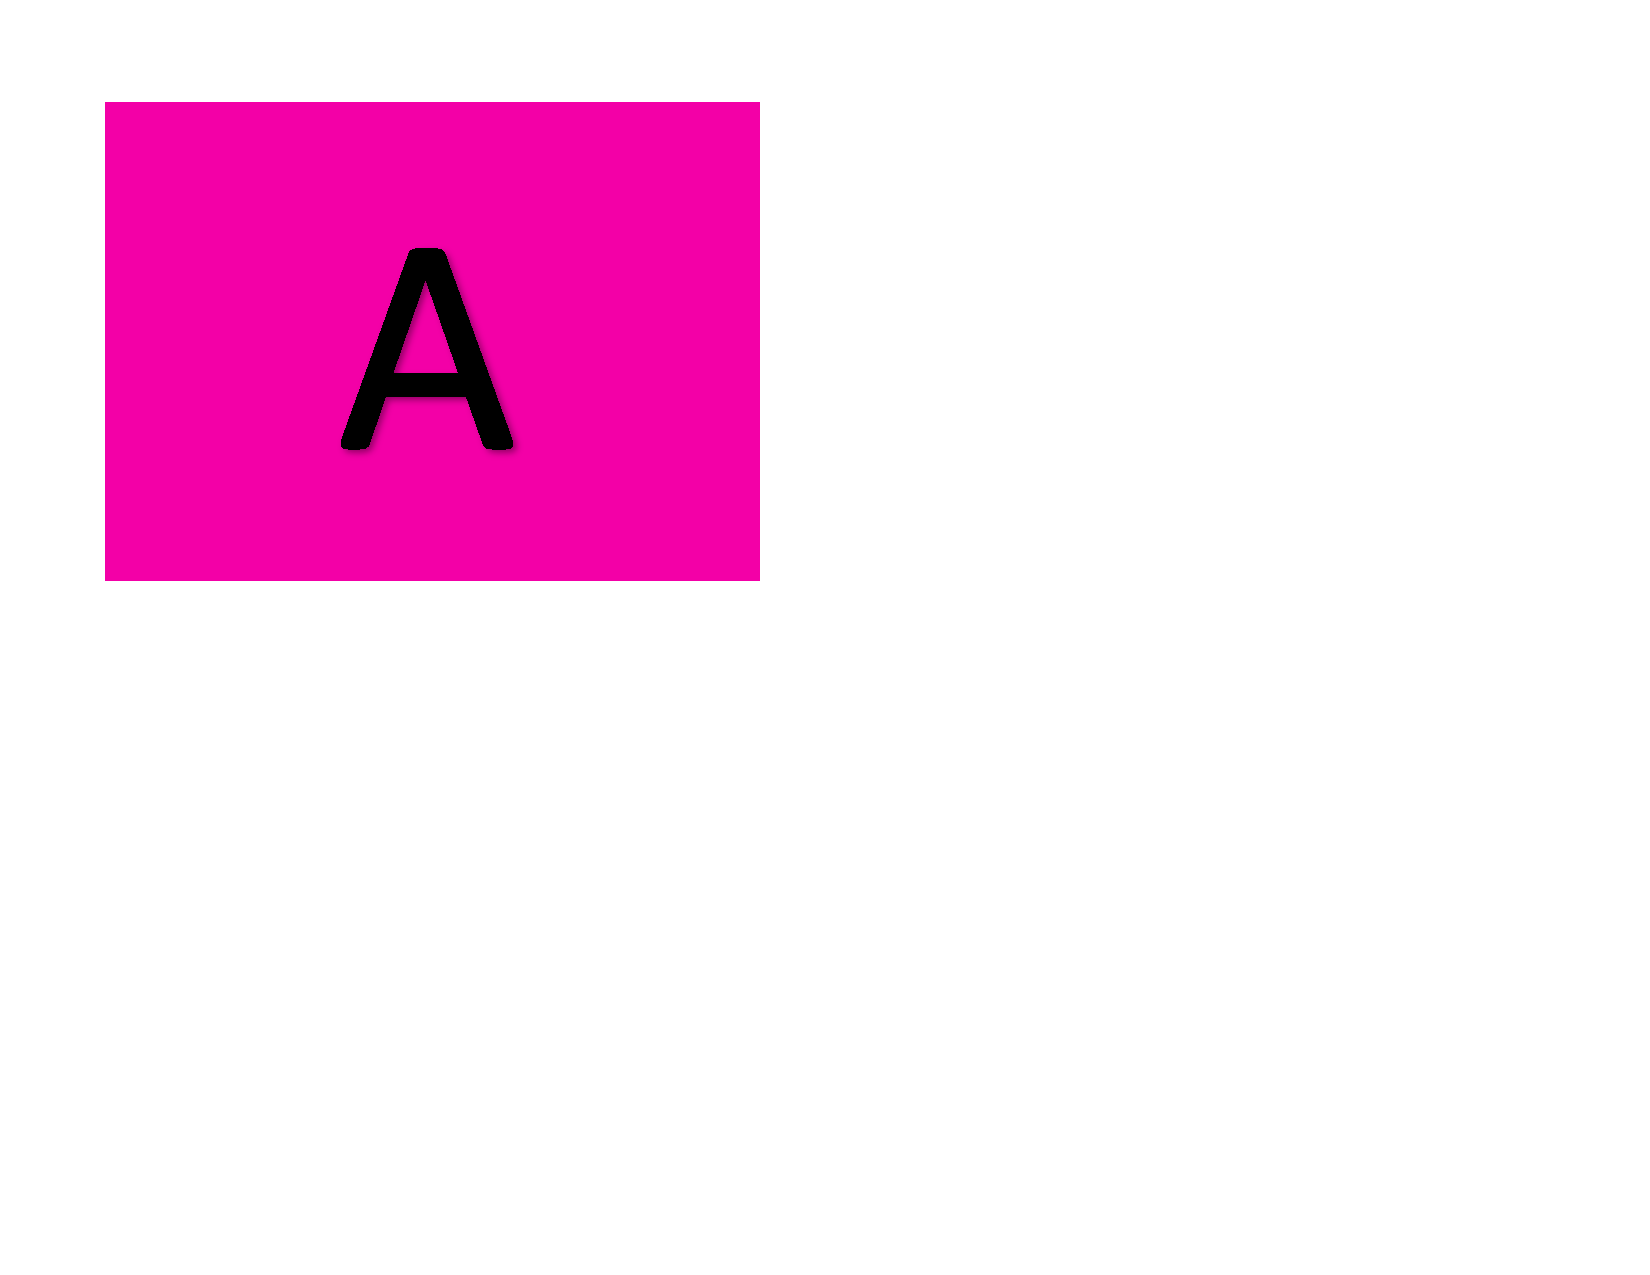
\includegraphics[width=0.8cm,height=0.5cm]{../../Lectures/figures/A}} ]  }
\newcommand*{\bitem}{ \item[{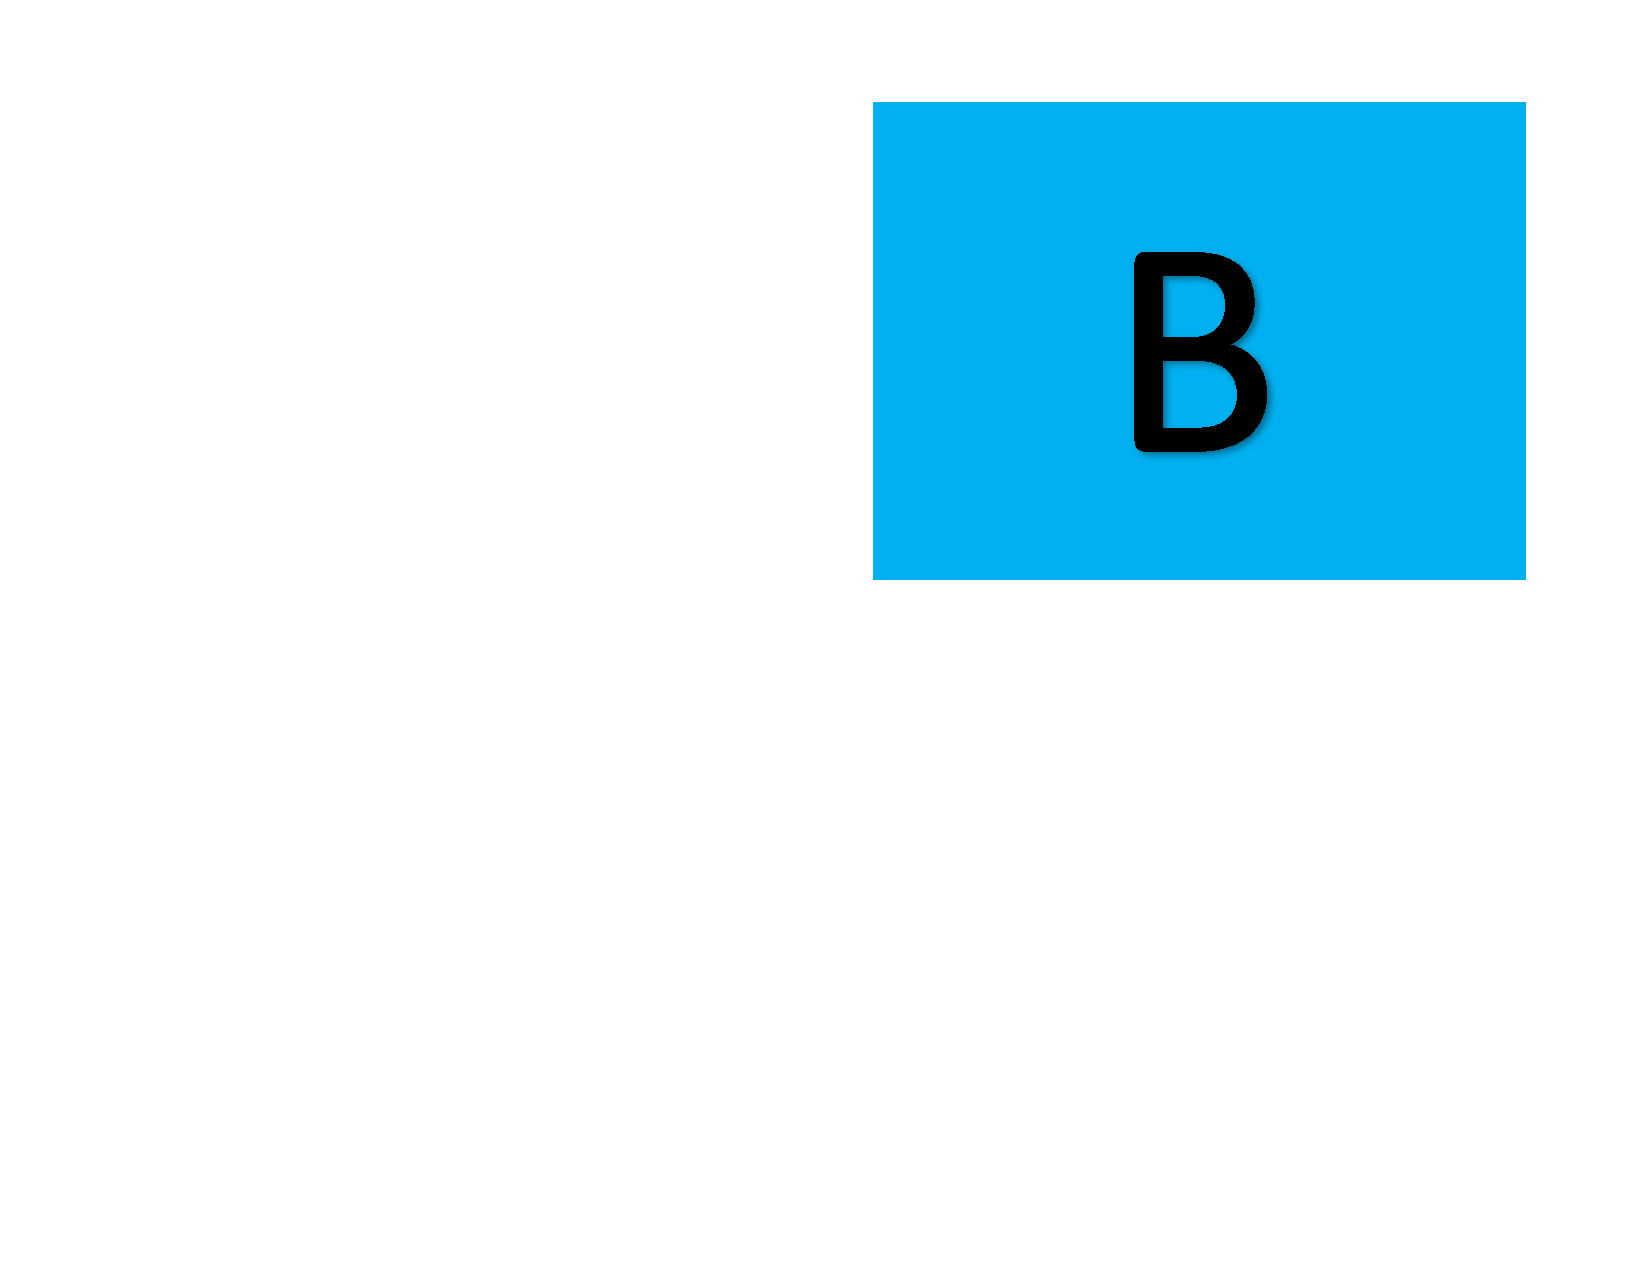
\includegraphics[width=0.8cm,height=0.5cm]{../../Lectures/figures/B}} ]  }
\newcommand*{\citem}{ \item[{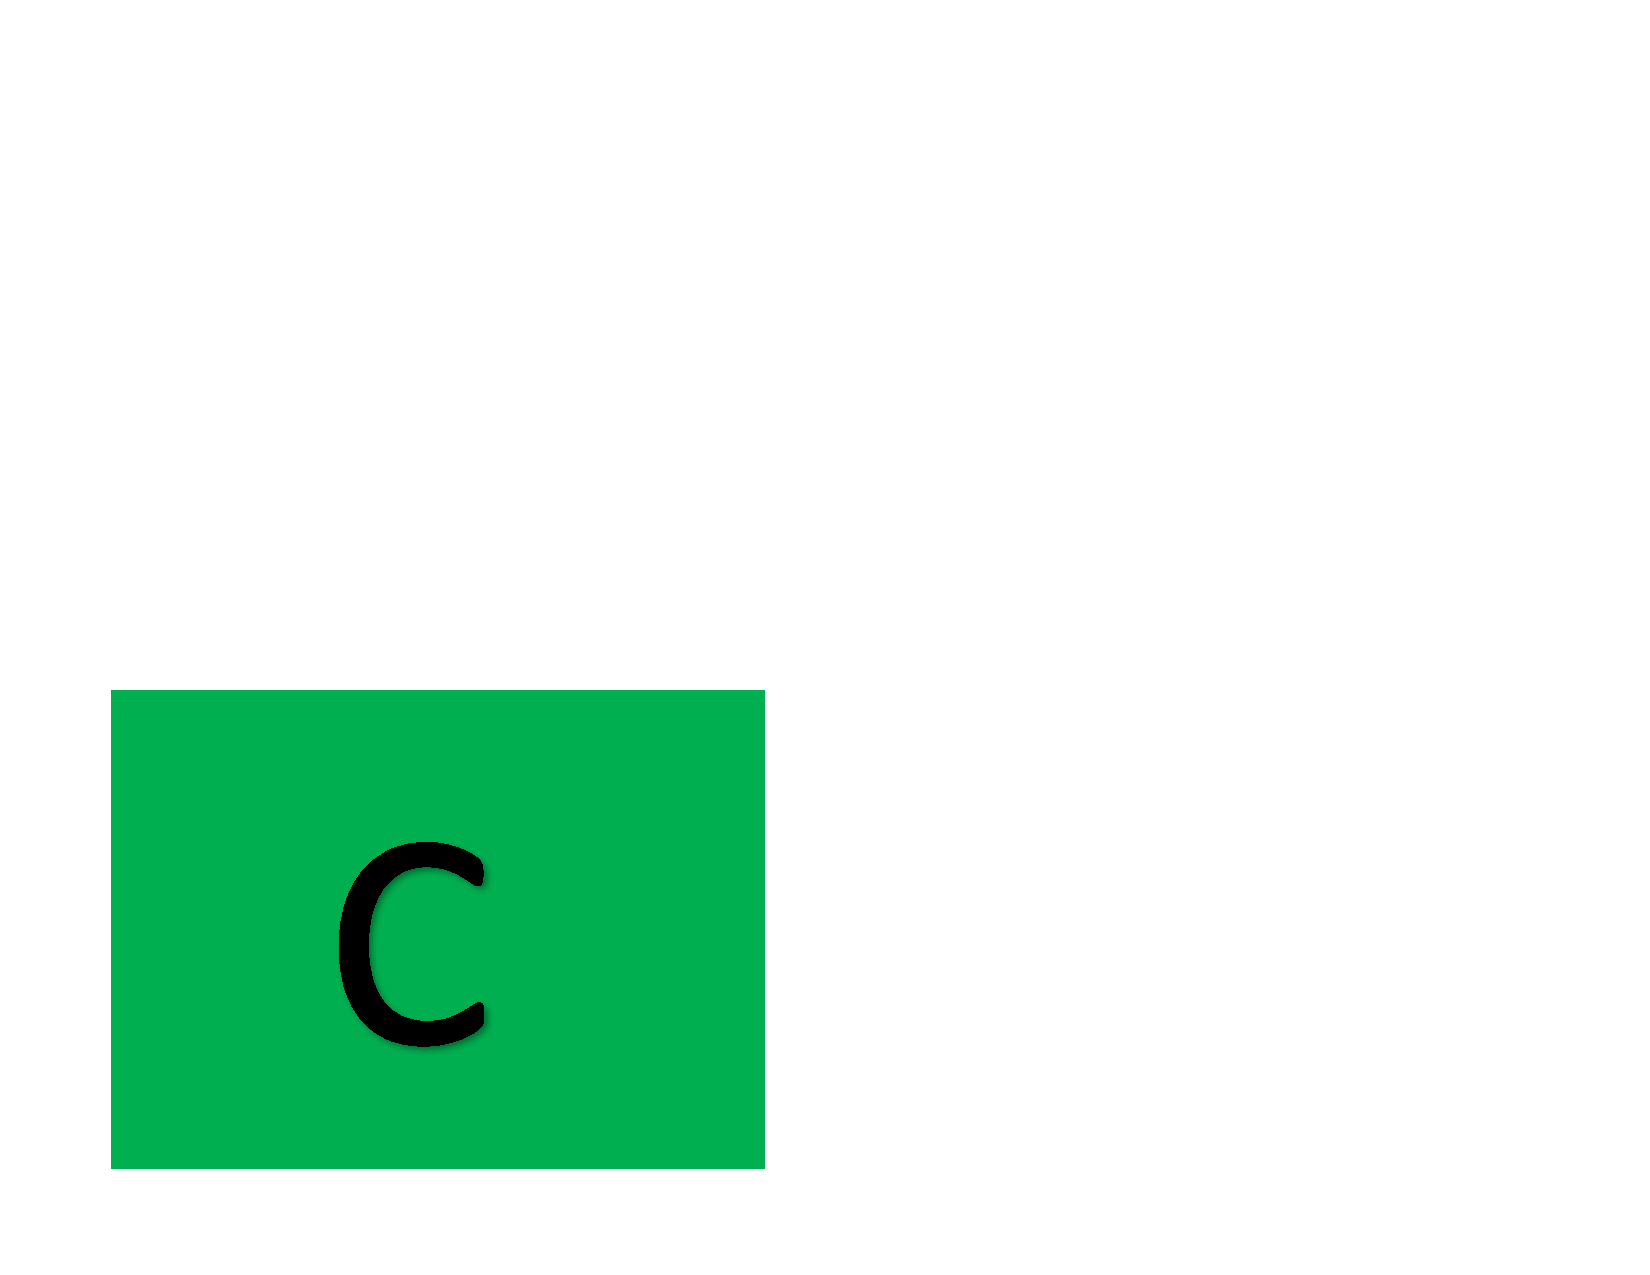
\includegraphics[width=0.8cm,height=0.5cm]{../../Lectures/figures/C}} ]  }
\newcommand*{\ditem}{ \item[{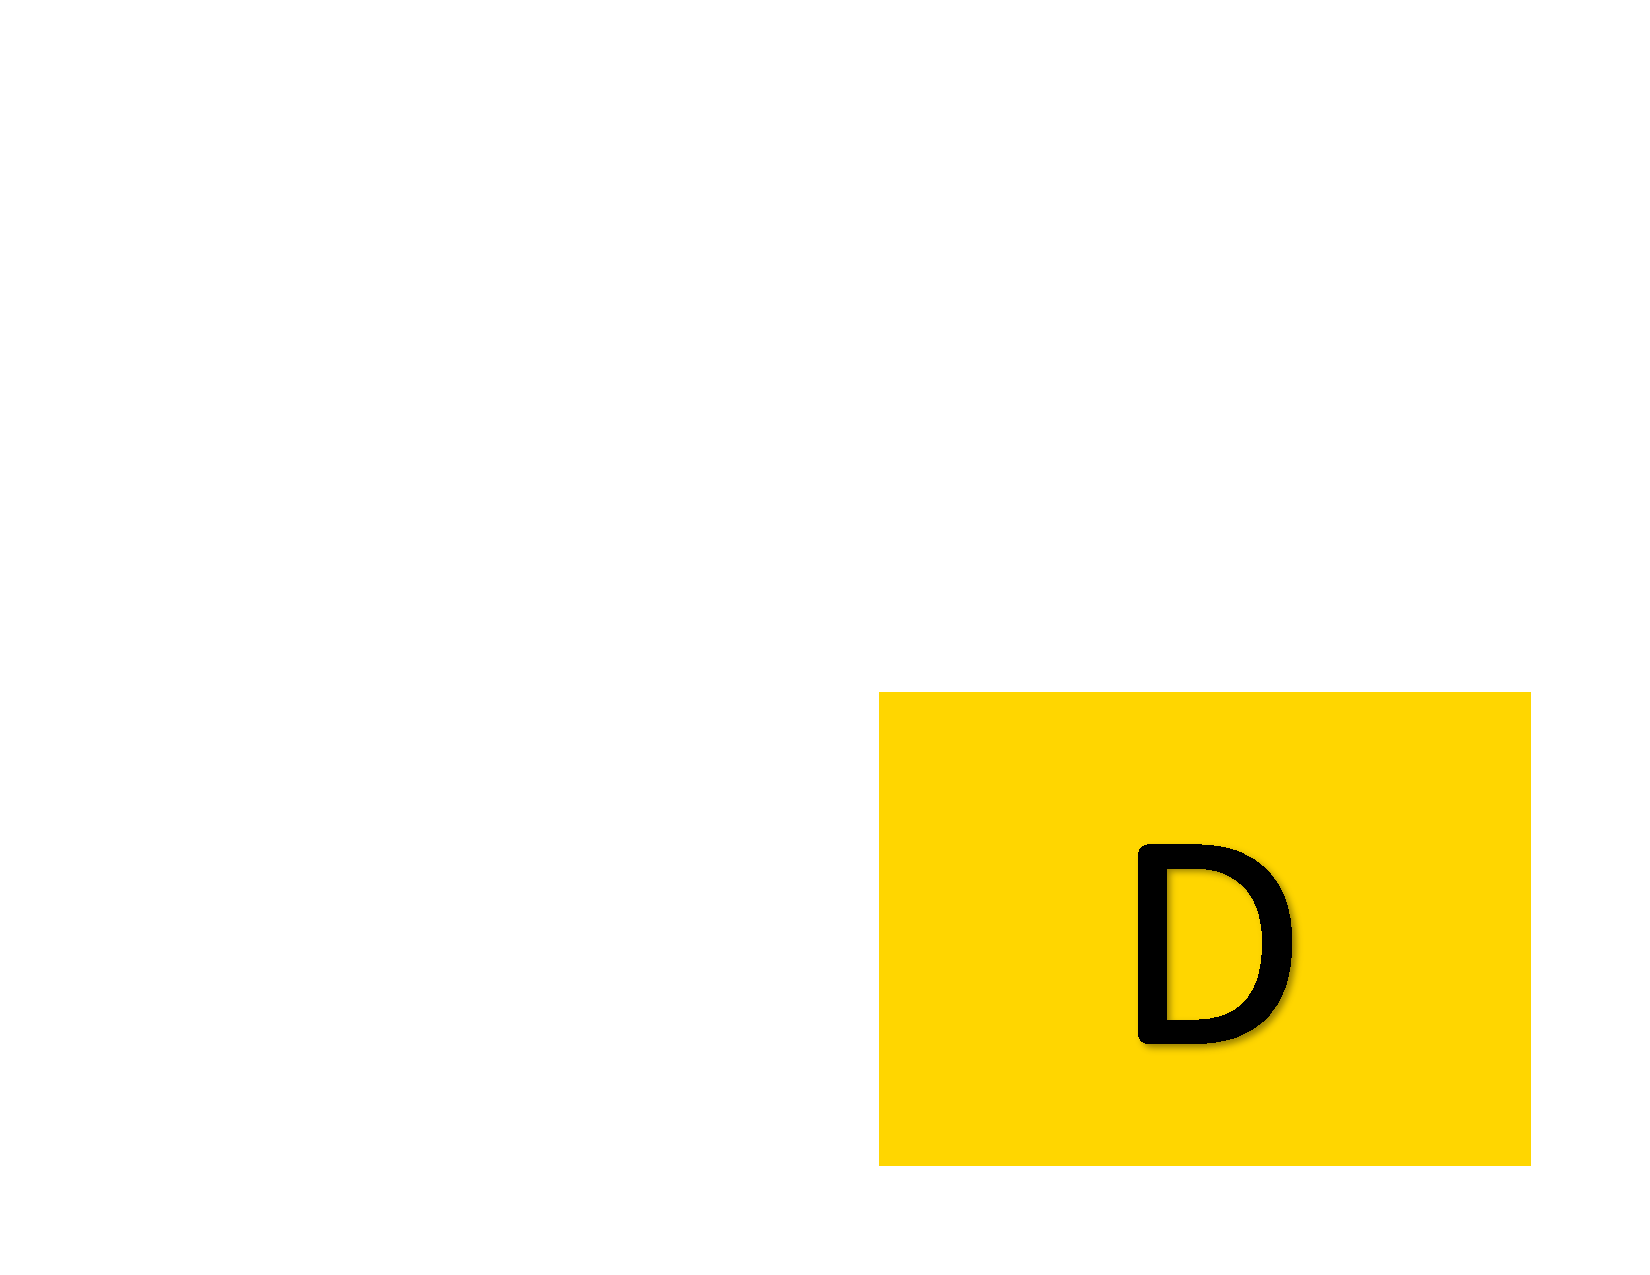
\includegraphics[width=0.8cm,height=0.5cm]{../../Lectures/figures/D}} ]  }
\newcommand*{\eitem}{ \item[{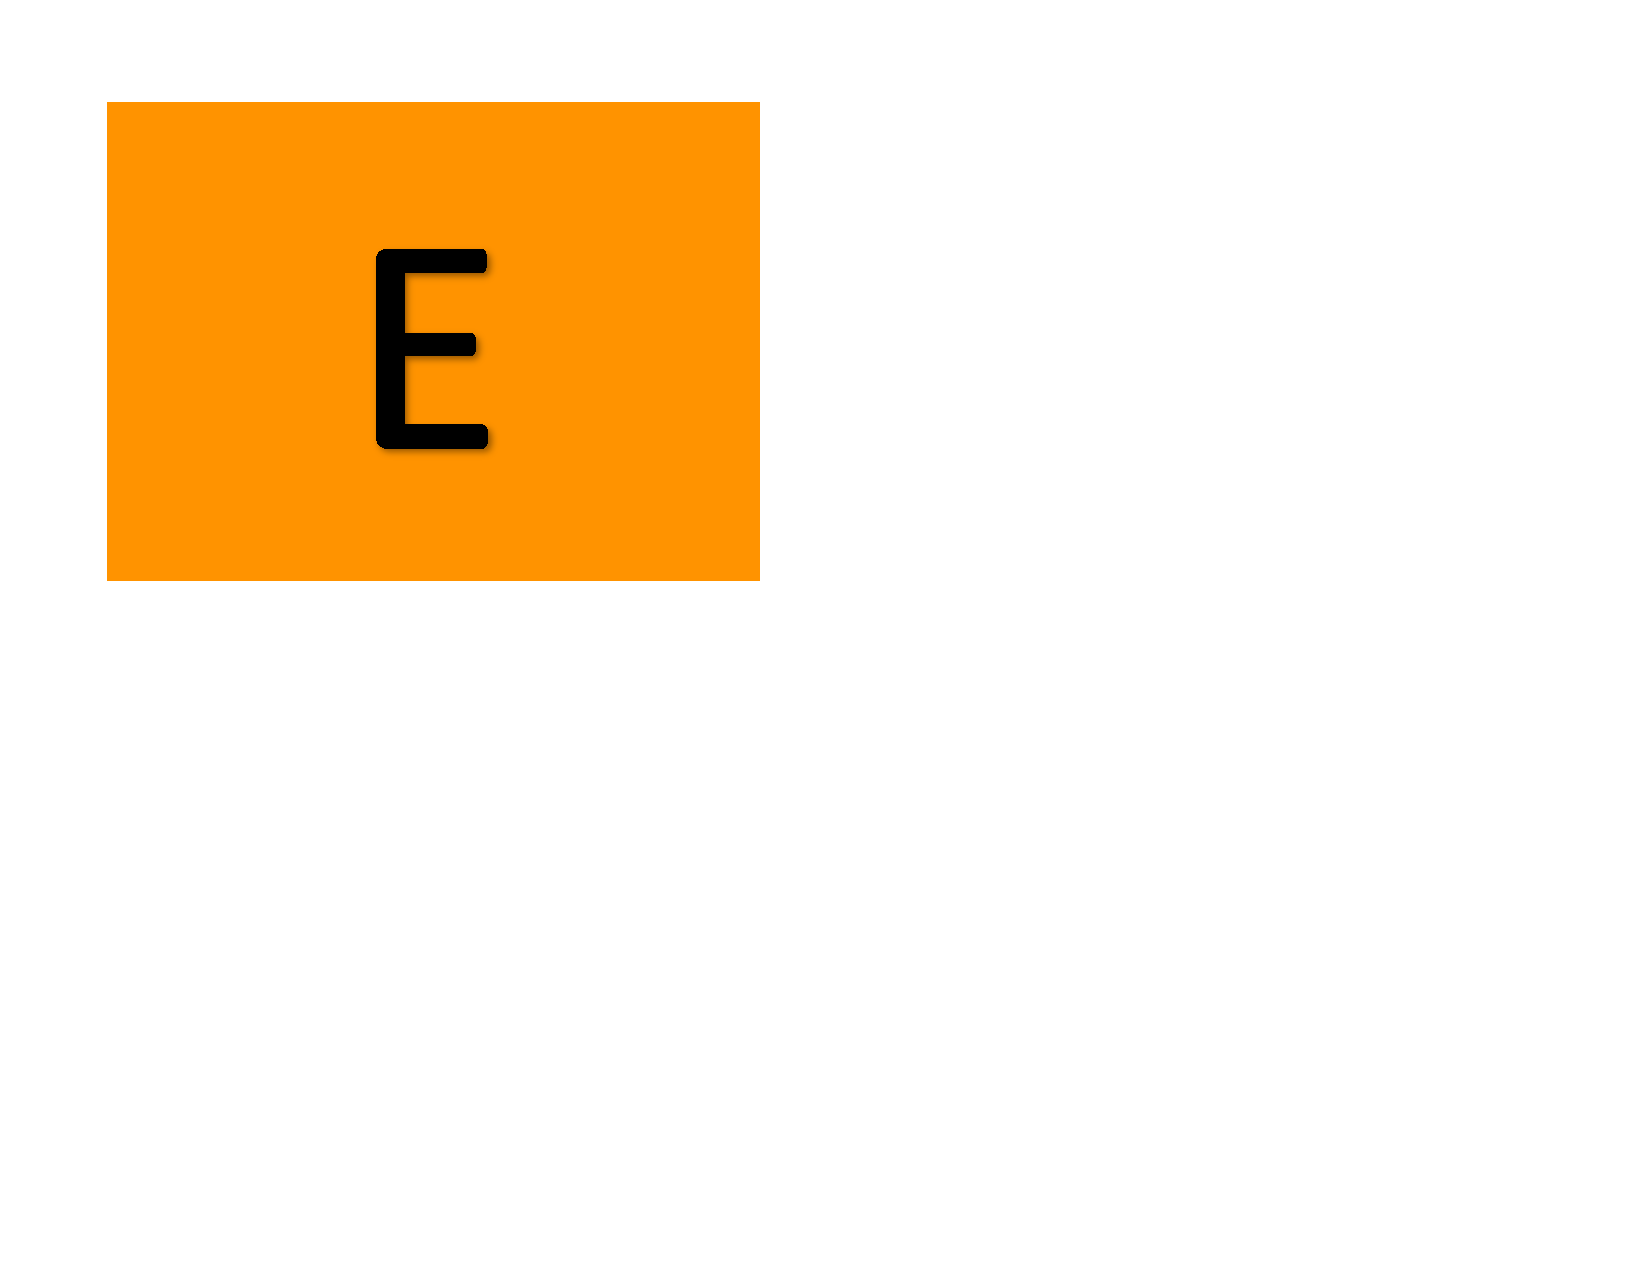
\includegraphics[width=0.8cm,height=0.5cm]{../../Lectures/figures/E}} ]  }
\newcommand*{\fitem}{ \item[{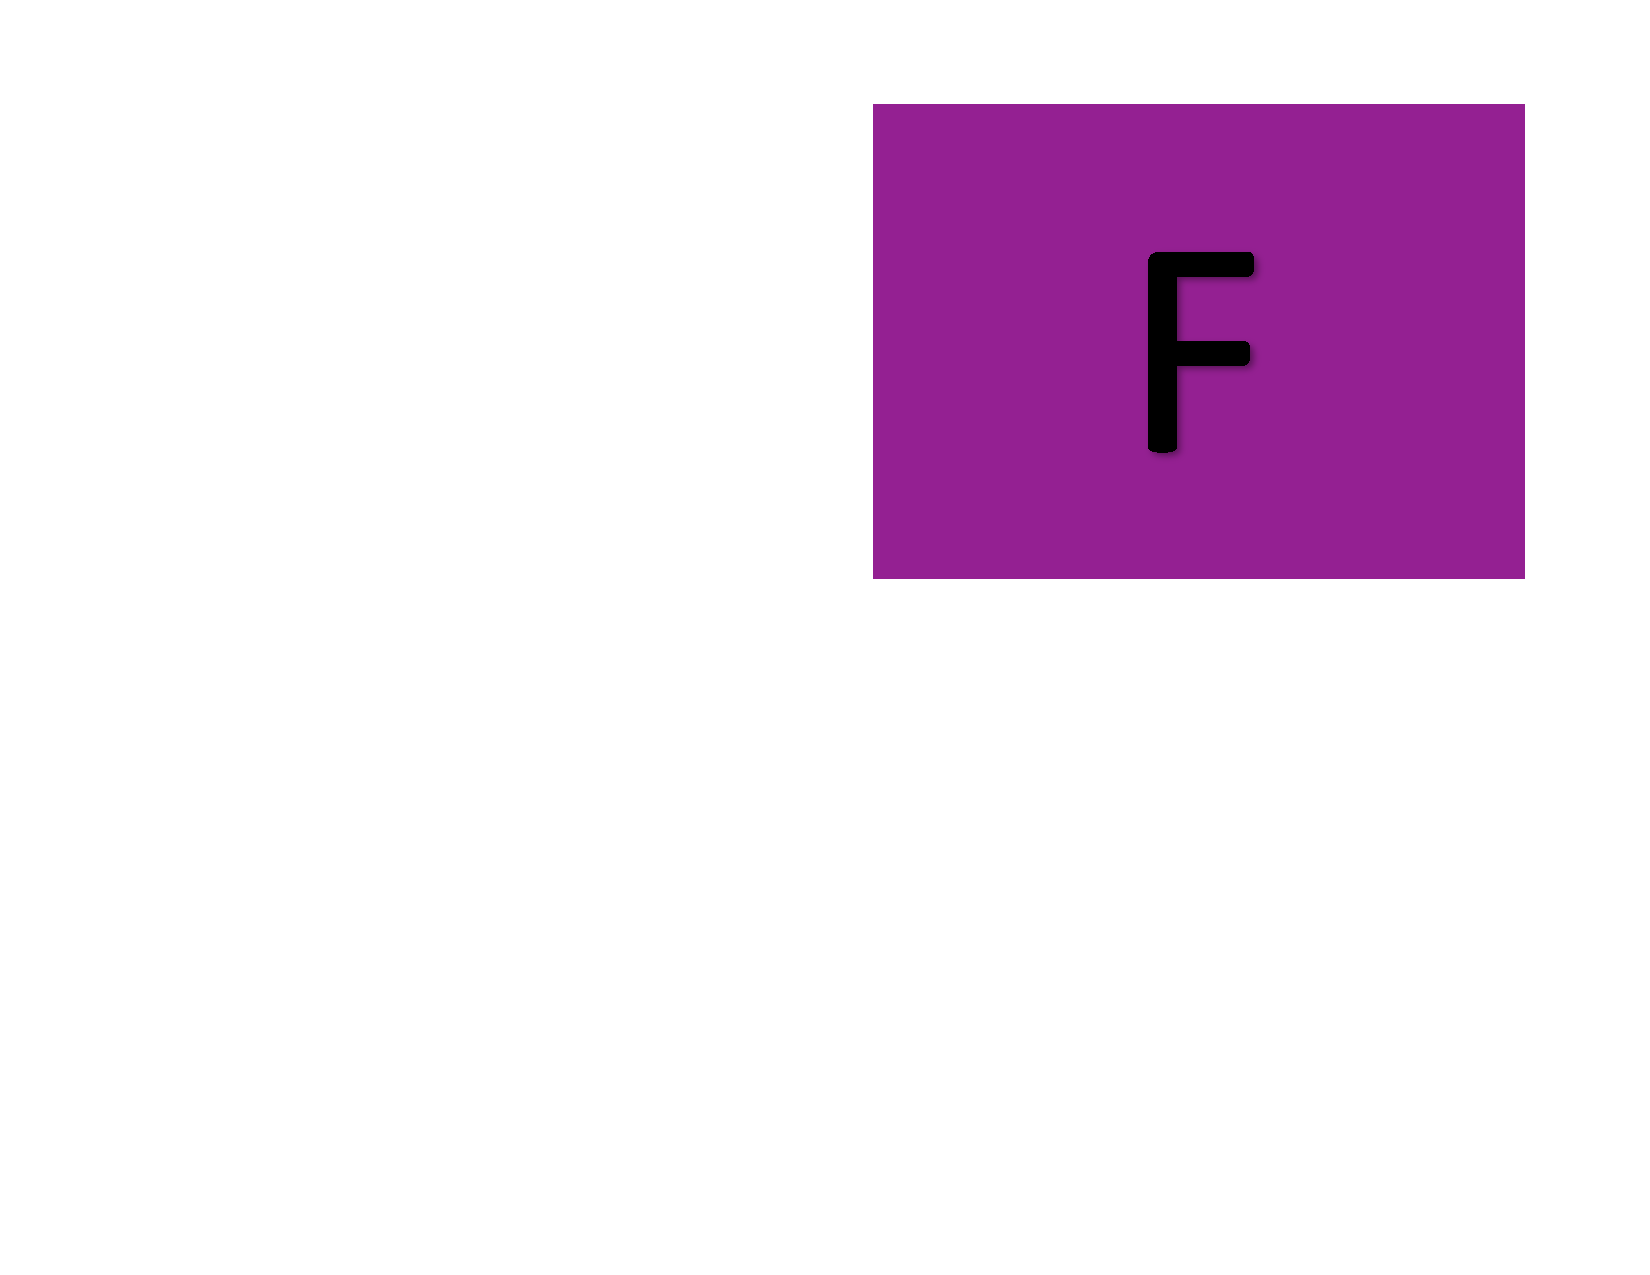
\includegraphics[width=0.8cm,height=0.5cm]{../../Lectures/figures/F}} ]  }


\newcommand{\hide}[1]{\underline{\phantom{#1 #1}}}

\usepackage{setspace}

\onehalfspacing

\begin{document}
	
	
	\lecture{10: Graph Algorithms: BFS and DFS}{February 20}
	
	\paragraph{Course Logistics}
	
	\begin{itemize}
		\item Graph algorithms: Chapter 22
		\item Homework 4 out this weekend, due next Friday
	\end{itemize}
	
	\section{Graph Representation}
	Consider a graph $G = (V,E)$ with a fixed node ordering $V = \{1, 2, \hdots , n\}$.
	
	\paragraph{Adjacency Matrix}
	The \textbf{adjacency matrix} $\mA$ of $G$ is defined so that
	
	\vspace{7cm}
	
	\paragraph{Adjacency List}
	The \textbf{adjacency list} Adj of $G$ is 
	
	\newpage 
	
	\subsection*{Graph Activity}
	Consider the following graph:
	
	\vs{8cm}
	
	
	\begin{itemize}
		\item Write down the adjacency matrix
		\item Write down the adjacency list 
		\item Write down the degree of each node
		\item Write down the neighborhood of node $3$
		\item Find the number of connected components
	\end{itemize}
	\begin{Qu}
		Assume that $G = (V,E)$ is a graph in which each node has at least one edge touching it. Let $n = |V|$ and $m = |E|$. How much space is needed to store the graph?
		\begin{itemize}
			\aitem $O(n)$ 
			\bitem $O(m)$
			\citem $O(n^2)$
			\ditem $O(mn)$
		\end{itemize}
	\end{Qu}
	\newpage
	
	\section{Breadth First Search}
	\textbf{Shortest Path Problem:} Given a graph $G = (V,E)$ and source node $s \in V$, find the shortest path from  $s$ to every other $v \in V$. \\
	
	%\begin{itemize}m  
	%	\item Find \emph{how far} away each node is from $s$
	%	\item Find \emph{shortest path} between $s$ and other nodes
	%\end{itemize}
	
	We will do this using the \emph{breadth first search} algorithm.
	
	\begin{tabular}{| l | p{8cm} | p{6cm} |}
		\hline
		Attribute & Explanation &Initialization \\
		\hline
		$u.\text{status}$ & tells us whether a node is \phantom{a a a undiscovered} \phantom{discovered}  \phantom{explored} &  \\
		\hline
		$u.\text{dist}$ & \phantom{distance from node $s$ a a a a a a a a space here}
		\phantom{for more writing later on in the dell you know}&  \\
		\hline
		$u.\text{parent}$ & \phantom{predecessor/``discoverer" of $u$ s a a a a a  here} \phantom{for more writing later on in the dell you know}& \\
		\hline
	\end{tabular}
	
	\vs{.25cm}
	We will also make use of \\ %a queue $Q$. 
	
	\textbf{Basic Idea}
	\begin{itemize}
		\item Mark $s$ as %discovered
		\item Iteratively \emph{explore} discovered nodes %to find new \emph{discovered} nodes
		\item Continuously update %distance from $s$ for each discovered node
	\end{itemize} 
	\textbf{Example}
	\vs{1cm}
	
	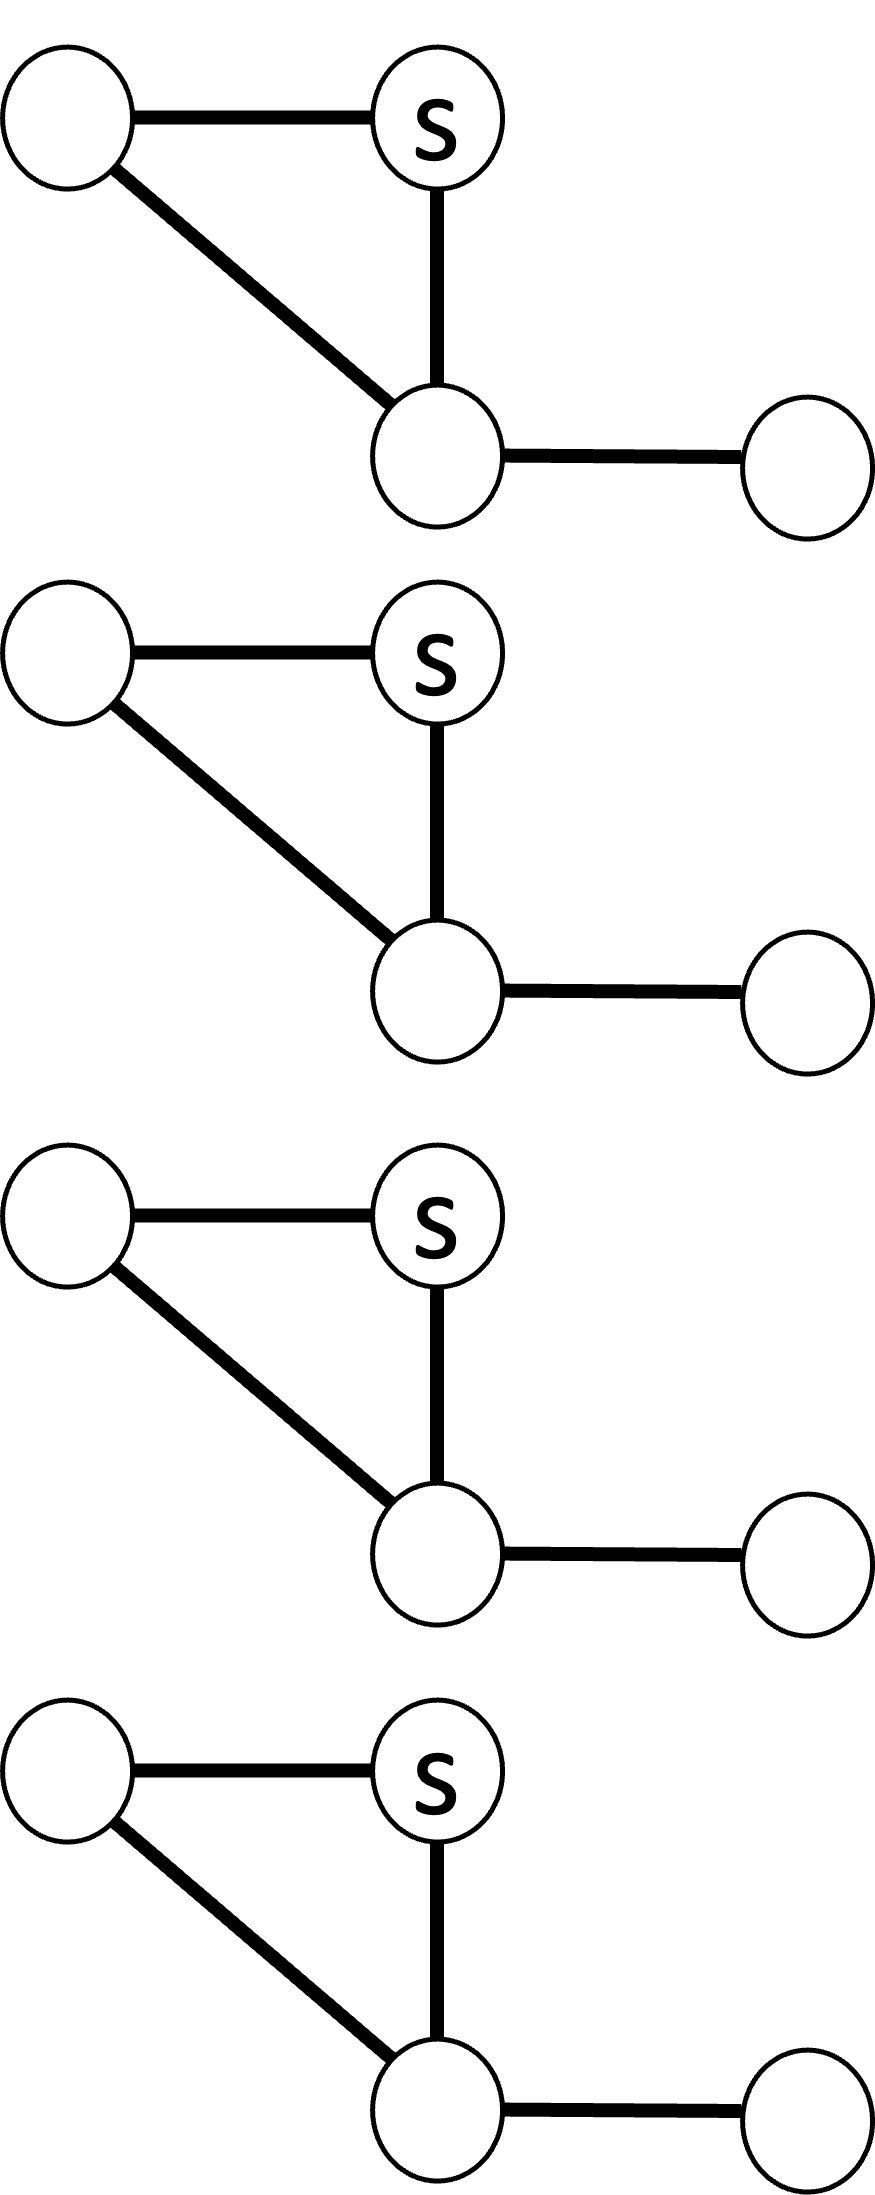
\includegraphics[width = .25\linewidth]{graphs1.png}
	\newpage
	
	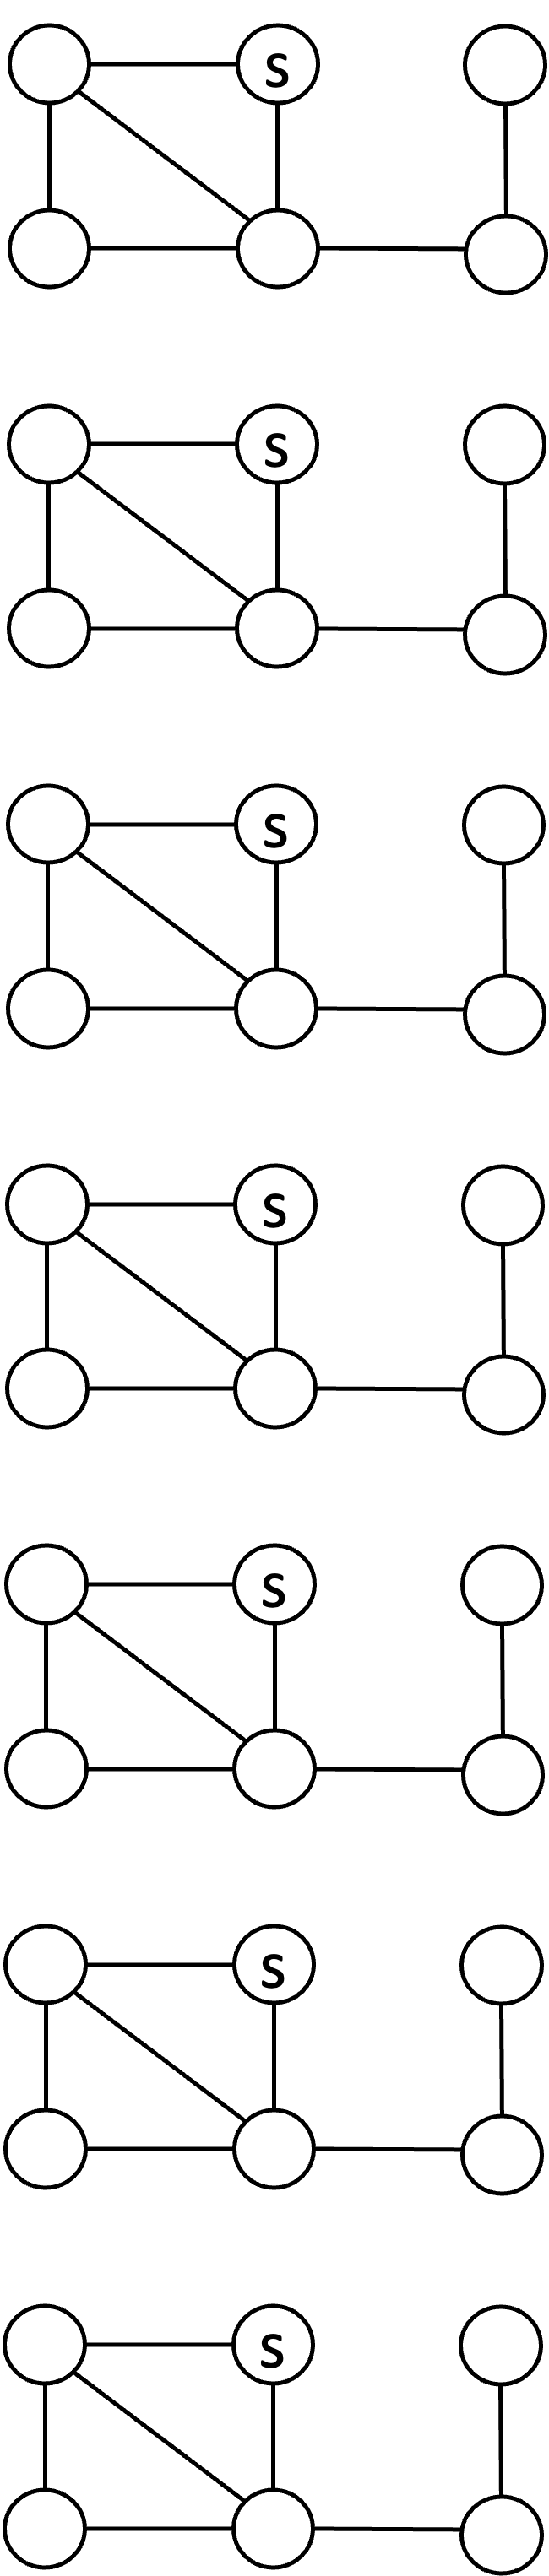
\includegraphics[width = .35\linewidth]{graphs2.png}
	
	\subsection{Shortest Paths and Breadth First Trees}
	\begin{definition}
		Given a graph $G = (V,E)$, source node $s$, and a \emph{parent} attribute for each node, a \hide{predecessor tree} is a subgraph $\hat{G} = (\hat{V}, \hat{E})$ where
		
		\vs{3cm}
		%		\begin{align*}
		%%			\hat{V} &= \{s\} \cup \{v \in V \colon v.\text{parent} \neq NIL \}\\
		%%			\hat{E} &= \{ (v.\text{parent}, v)  \colon v \in \hat{V} - \{s\} \}
		%		\end{align*}
		
		It is furthermore a \hide{breadth-first tree} if it contains a unique simple path \\
		
		from $s$ to $v$ that is \hide{the shortest path from $s$ to $v$ in $G$.} \\
	\end{definition}
	
	\textbf{Benefits of the BFS algorithm}
	\begin{itemize}
		\item If $G$ is undirected, it finds the \hide{connected component that} \\%$s$ is in
		\item It tells us the \hide{shortest path (and distance) from $s$ }\\ %to each node
		\item It provides a \hide{breadth-first tree} 
	\end{itemize}
	
	
	
	
	\newpage
	
	\subsection{Code and Runtime Analysis}
	\begin{algorithm}[t]
		\textsc{BFS}($G$,$s$)
		\begin{algorithmic}
			\For{$v \in V $}
			\State $v.\text{parent} = NIL$
			\State $v.\text{dist} = \infty$
			\State $v.\text{status} = \text{U}$
			\EndFor
			\State $s.\text{dist} = 0$
			\State $s.\text{status} = \text{D}$
			\State Initialize $Q$
			\State $\text{Enqueue}(s)$
			\While{$|Q| > 0$}
			\State $u = \text{Dequeue}(Q)$
			\State $N(u) = \text{Adj}[u]$
			\For{$v$ in $N(u)$}
			\If{$v.\text{status} == U$}
			\State $v.\text{status} = D$
			\State $v.\text{parent} = u$
			\State $v.\text{dist} = u.\text{dist} + 1$
			\State $\text{Enqueue}(v)$
			\EndIf
			\EndFor
			\State $u.\text{status} = E$
			\EndWhile
		\end{algorithmic}
	\end{algorithm}
	
	
	\begin{itemize}
		\item We assume $G$ is undirected and stored as an adjacency list.
		\item Initializing attributes takes \hide{$O(n)$ time}
		\item Each node $u$ only enters $Q$ once, and entering/leaving $Q$ takes \hide{$O(1)$}
		\item When we \emph{explore} $u$, we discover up to \hide{$d_u$ neighbors}
	\end{itemize}
	Using aggregate analysis, what is the overall runtime of this method? \\

	
	\newpage
	
	\section{Depth First Search: Background and Motivating problems}
	Recall that a \emph{breadth-first} search explores nodes that are $k$ steps away from node $s$ before exploring any nodes that are $k+1$ steps away. \\
	
	A \emph{depth-first search} instead explores the \emph{most recently discovered vertex} before backtracking and exploring other previously discovered nodes.\\
	
	Roughly speaking, this is accomplished by \hide{replacing the queue}. \\
	
	Depth first search is used in several applications for analyzing directed graphs. We will take a closer look at these applications before exploring how to solve them using DFS. \\
	
	\paragraph{Directed graph reminders}
	
	% path
	
	\newpage
	
	\subsection{Reachability and Connected Components}
	\textbf{Reachability.} Given a graph $G = (V,E)$ and node set $S \subseteq V$, node $v \in S$ is \emph{reachable} from node $u \in S$ if \hide{there is a path of nodes from $u$ to $v$}. \\
	\vfill
	
	
	\textbf{Connected components.} 
	For an undirected graph $G = (V,E)$ a connected component is a maximal subgraph in which every node in is \hide{reachable from every other } \\
	
	
	\vfill
	
	\textbf{Weakly Connected components} If $G = (V,E)$ is directed, a \emph{weakly connected component} is \hide{a connected component in the graph}\\ % obtained by ignoring edge directions. \\
	
	
	\vfill
	
	
	\textbf{Strongly Connected components} If $G = (V,E)$ is directed, a \emph{strongly connected component} is subgraph $S \subseteq V$ in which there is \hide{a directed path of nodes (in $S$)} \\ % every pair of nodes in $S$. 
	\vfill 
	
	\newpage
	
	\begin{Qu}
		How many weakly connected components and strongly connected components are there in the following graph, respectively?
		
		\begin{itemize}
			\aitem 1 and 3
			\bitem 1 and 2
			\citem 0 and 1
			\ditem 2 and 3
		\end{itemize}
		
	\end{Qu}
	
	
	\vs{3cm}
	
	\subsection{Directed Acyclic Graphs}
	A \emph{cycle} in a directed graph is a directed path \hide{that starts and ends at} \\ % the same node. \\
	
	\vs{2cm}
	
	
	A \emph{Directed acyclic} graph is a directed graph that \hide{has no cycles}.
	
	
	\paragraph{Examples}
	
	
	
	\newpage
	
	
	\subsection{Topological Sorting}
	A topologically ordering of a directed acyclic graph $G = (V,E)$ is an ordering of nodes so that: \\
	
	
	%for each edge  $(u,v) \in E$, $u$ comes before $v$ in the ordering.
	
	%	\paragraph{Examples and applications}
	
	\newpage 
	
	\section{Depth First Search Algorithm}
	Unlike in a BFS, a depth-first search (DFS):
	\begin{itemize}
		\item Explores the \emph{most recently discovered vertex} before backtracking and exploring other previously discovered vertices
		\item All nodes in the graph are explored (rather than just a DFS for a single node $s$)
		\item We keep track of a global \emph{time}, and each node is associated with two timestamps for when it is \emph{discovered} and \emph{explored}.
	\end{itemize}
	
	Each node $u \in V$ is associated with the following attributes
	
	\begin{tabular}{| l | p{8cm} | p{6cm} |}
		\hline
		Attribute & Explanation &Initialization \\
		\hline
		$u.\text{status}$ & tells us whether a node has been \emph{undiscovered}, \emph{discovered}, and \emph{explored} &  \\
		\hline
		$u.\text{D}$ & timestamp when $u$ is first discovered \phantom{the aa} \phantom{quick brown fox jumps over the lazy dog}
		\phantom{for more writing later on in the dell you know} &  \\
		\hline
		$u.\text{F}$ & timestamp when $u$ is finished being explored \phantom{the aa} \phantom{quick brown fox jumps over the lazy dog}
		\phantom{for more writing later on in the dell you know}  &  \\
		\hline
		$u.\text{parent}$ & predecessor/``discoverer" of $u$ \phantom{s a a a a a  here} \phantom{for more writing later on in the dell you know}& \\
		\hline
	\end{tabular}
	\newpage 
	
	%\section{Code and Example}
	
	\begin{minipage}[t]{0.45\textwidth}
		%	\begin{algorithm}
		\textsc{DFS}($G$)
		\begin{algorithmic}
			\For{$v \in V $}
			\State $v.\text{parent} = NIL$
			\State $v.\text{status} = \text{U}$
			\EndFor
			\State $\text{time} = 0$
			\For{$u \in V$}
			\If{$u.\text{status} == U$}
			\State $\textsc{DFS-Visit}(G,u)$
			\EndIf
			\EndFor
		\end{algorithmic}
		%	\end{algorithm}
	\end{minipage}
	\begin{minipage}[t]{0.45\textwidth}
		%	\begin{algorithm}
		\textsc{DFS-Visit}($G,u$)
		\begin{algorithmic}
			\State $\text{time} = \text{time} + 1$
			\State $u.D = \text{time}$
			\State $u.\text{status} = D$
			\For{$v \in \text{Adj}[u]$}
			\If{$v.\text{status} == U$}
			\State $v.\text{parent} = u$
			\State $\textsc{DFS-Visit}(G,v)$
			\EndIf
			\EndFor
			\State $u.\text{status} = \text{E}$
			\State $\text{time} = \text{time} + 1$
			\State $u.F = \text{time}$
		\end{algorithmic}
		%	\end{algorithm}
	\end{minipage}
	\vspace{1cm}
	
	\includegraphics[width = .4\linewidth]{dfs.png}
	\newpage 
	
	\newpage
	\subsection{Runtime Analysis}
	\begin{Qu}
		What is the runtime of a depth first search, assuming that we store the graph in an adjacency list, and assuming that $|E| = \Omega(|V|)$?
		\begin{itemize}
			\aitem $O(|V|)$
			\bitem $O(|E|)$
			\citem $O(|V| \times |E|)$
			\ditem $O(|V|^2)$
			\eitem $O(|E|^2)$
		\end{itemize}
	\end{Qu}
	\newpage
	\subsection{Properties of DFS}
	
	\begin{theorem}
		In any depth-first search of a graph $G = (V,E)$, for any pair of vertices $u$ and $v$, exactly one of the following conditions holds:\\ \\
		\begin{itemize}
			\item $[u.D,u.F]$ and $[v.D, v.F]$ are disjoint; \hide{neither of $u$ or $v$ is a} \\
			\item $[v.D, v.F]$ contains $[u.D,u.F]$ and \hide{$v$ is a descendant of $u$} \\
			\item $[u.D,u.F]$ contains $[v.D, v.F]$ and \hide{$u$ is a descendant of $v$}
		\end{itemize}
	\end{theorem}
	
	\vs{2cm}
	
	
	\newpage
	\subsection{Classification of Edges}
	
	Given a graph $G = (V,E)$ performing a DFS on $G$ produces a graph $\hat{G} = (V, \hat{E})$ where
	\begin{align*}
		\hat{E} = \{ (u.\text{parent}, u) \colon v \in V \text{ and } v.\text{parent} \neq NIL  \}
	\end{align*}
	This is called a \emph{depth-first} forest of $G$. \\
	
	\vspace{4cm}
	
	Given any edge $(u,v) \in E$, we can classify it based on the status of node $v$ when we are performing the DFS:\\
	
	
	\begin{tabular}{| l | p{8cm} | p{6cm} |}
		\hline
		Edge & Explanation & How to tell when exploring $(u,v)$? \\
		\hline
		\textbf{Tree edge}  & edge in $\hat{E}$ & %$v.\text{status} == U$ 
		\\
		\hline
		\textbf{Back edge} & connects $u$ to ancestor $v$ & %$v.\text{status} == D$ 
		\\
		\hline
		\textbf{Forward edge} & connects vertex $u$ to descendant $v$ & \phantom{spaceasdfasdf2xsdf} \emph{and} $u.D < v.D$\\
		\hline
		\textbf{Cross edge} & either (a) connects two different trees or (b) crosses between siblings/cousins in same tree &  \phantom{spaceasdfasdf2xsdf} \emph{and} $u.D > v.D$\\
		\hline
	\end{tabular}
	
	%We can define four types of edges in terms of the depth-first forest $\hat{G}$:
	%\begin{enumerate}
	%	\item \textbf{Tree edges}: edges from $\hat{E}$
	%	\item \textbf{Back edges}: edges $(u,v)$ where $v$ is an ancestor of $u$ in a DFS tree
	%	\item \textbf{Forward edges}: edges $(u,v)$ where $v$ is a descendant of $u$ in a DFS tree
	%	\item \textbf{Cross edges}: all other edges. Either edges between vertices in the same DFS tree, or between different DFS trees.
	%\end{enumerate}
	\newpage
	\section{Practice}
	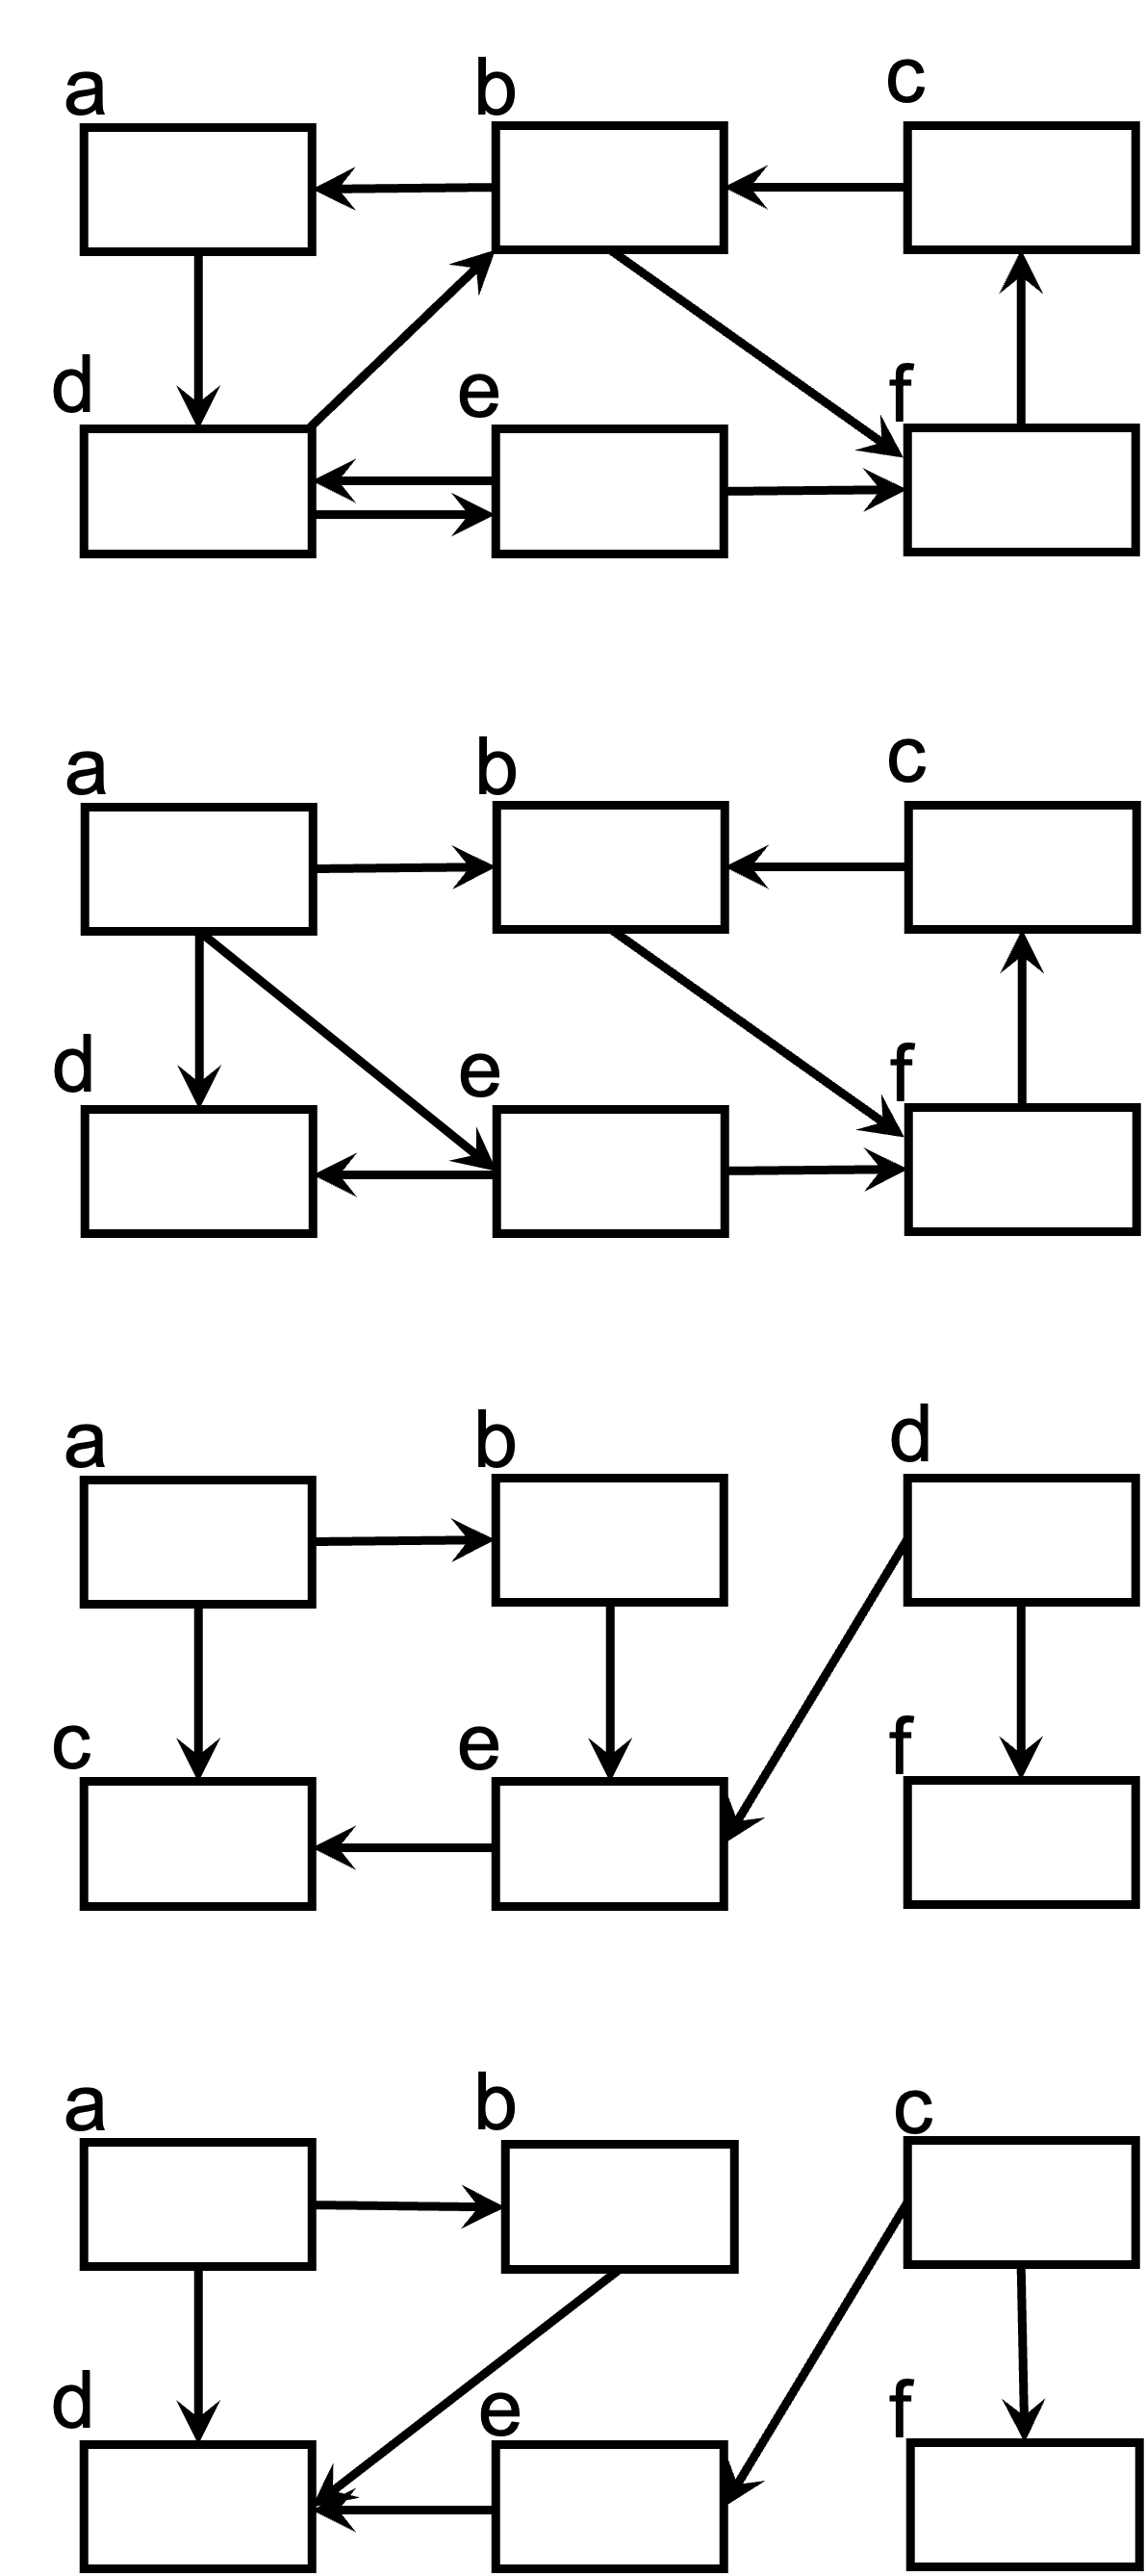
\includegraphics[width = .6\linewidth]{manydfs.png}
	\newpage
	\begin{Qu}
		How many of the above graphs were directed acyclic graphs?
		\begin{itemize}
			\aitem 1
			\bitem 2
			\citem 3
			\ditem 4
			\eitem none of them
		\end{itemize}
	\end{Qu}
	
\end{document}


\newpage
Most important things to learn about BFS:
\begin{itemize}
	\item How to perform a BFS on a node in a graph (e.g., provide pseudocode, or find a breadth-first tree for an example graph)
	\item What are the benefits of a BFS---what does it provide and what problems does it solve?
	\item What is the computational complexity of running a breadth first search, and roughly speaking, why?
\end{itemize}